\documentclass[letterpaper, 10 pt, conference]{ieeeconf}

\IEEEoverridecommandlockouts                              % This command is only
                                                          % needed if you want to
                                                          % use the \thanks command
\overrideIEEEmargins
% See the \addtolength command later in the file to balance the column lengths
% on the last page of the document

% The following packages can be found on http:\\www.ctan.org
\usepackage{graphicx} % for pdf, bitmapped graphics files
\usepackage{epsfig} % for postscript graphics files
\usepackage{mathptmx} % assumes new font selection scheme installed
\usepackage{times} % assumes new font selection scheme installed
%\usepackage{amsmath} % assumes amsmath package installed
%\usepackage{amssymb}  % assumes amsmath package installed

%%%%%%%%%%%%%%%%%%%%%%%%%%%%%%%
% added packages 
%\usepackage {hyperref}
\usepackage {subfig}
\usepackage {xspace}
%% Math and symbol packages
\usepackage{amssymb}
\usepackage{amsmath}
%%% for kmap tables:
%\usepackage{hhline}
\usepackage{multicol}
%%% for \dashline
%\usepackage{epic}
\usepackage {enumerate}
\usepackage{scalefnt}
%\usepackage{enumitem}
%%%%%%%%%%%%%%%%%%%%%%%%%%%%%%%%


% for cool graphics
\usepackage{pgf,tikz}
\usetikzlibrary{arrows,shapes.symbols,shapes.callouts,snakes,shapes.geometric}
\hyphenation{}



% Process this with:
% pdflatex latex-template.tex
% bibtex latex-template.bib
% pdflatex latex-template.tex
% pdflatex latex-template.tex
\begin{document}



\title{
Gr{\H o}bner Basis Computation for Boolean Rings Using Zero Suppressed Binary Decision Diagrams
}

\author{Revanth Rajalbandi, Harsha Gadiraju and Ian Noy\\
 	\textit{Dept. of Electrical and Computer Engineering, University of Utah}\\
 	\textit{revanth.rajalbandi@utah.edu, harsha.gadiraju@utah.edu, ian.noy@utah.edu}
}
\maketitle



%%%%%%%%%%%%%%%%%%%%%%%%%%%%%%%%%%%%%%%%%%%%%%%%%%%%%%%%%%%%%%%%%%%%%%%%%%%%%%%%

\begin{abstract}
Zero Suppressed Binary Decision Diagrams (ZBDDs) are an efficient way to represent and manipulate sets of sets problems. As an ideal is a set of polynomials and each polynomial is a set of monomials, ZBDDs can manipulate these sets and yield faster results when compared to traditional BDDs used in equivalence checking of circuits. ZBDDs encode the functionality of the circuit and so does the Gr{\H o}bner basis. Here the overall idea is to implement Gr{\H o}bner basis using ZBDDs with the help of CUDD package (CUDD is a BDD package written in C which implements BDDs and ZBDDs) \cite{somenzi1998cudd}.  This paper describes the algorithm of Gr{\H o}bner basis computation for boolean rings using Zero Suppresed Binary Decision Diagrams and three cases to test the implementation.  The results achieve the desired reduced Gr{\H o}bner basis forms.
\end{abstract}

%%%%%%%%%%%%%%%%%%%%%%%%%%%%%%%%%%%%%%%%%%%%%%%%%%%%%%%%%%%%%%%%%%%%%%%%%%%%%%%%



\section{Introduction}
\label{sec:intro}
Zero-suppressed BDDs are a new type of BDD adapted for representing sets of combinations. They are based on the following reduction rules.

\begin{itemize}
	\item Eliminate all nodes with the 1-edge pointing to the 0-terminal node. Then connect the edge to the other subgraph directly.
	\item Share all the equivalent sub-graphs in the same manner as with the conventional BDDs.
\end{itemize}

Notice that, contrary to conventional BDDs, we do not eliminate nodes whose two edges both point to the same node. This reduction rule is asymmetric for the two edges as the nodes remain when their 0-edge points to a terminal node. When the number and order of the variables are fixed, 0-suppressed BDDs provide canonical forms of Boolean Functions.

Here, we document our attempt at implementing the Buchberger's algorithm on ZBDDs.  This is not an original idea, the same type of research has been performed in the PolyBori program \cite{brickenstein2009polybori}.  PolyBori provides a Gr{\H o}bner basis framework for Boolean polynomials. This paper introduces the concept of generating Gr{\H o}bner basis computations on ZBDDs.  The authors also use the CUDD package to manipulate ZBDDs.  The purpose of their research is to provide a solution to the problem which is formal verification.  There are many ways to verify circuits and running the Buchberger's algorithm on polynomials is an efficient solution.  ZBDDs are simplified sets of combinations that can represent polynomials.  Combining these ideas into a general model could provide a faster and more efficient means towards formal circuit verification.
\section{CUDD Package}
\label{sec:cudd}

Colorado University Decision Diagram (CUDD) is a software package that was developed by Fabio Somenzi at the University of Colorado at Boulder \cite{somenzi1998cudd}.  The package is capable of manipulating BDDs, Algebraic Decision Diagrams (ADDs) and ZBDDs with many sets of operations.  These objects can also be converted from one form to another in a seamless manner.  When building a ZBDD it is important to treat the function as a set.  Here is an example of how a ZBDD is built in CUDD package.
\begin{align*}
&//\ First\ create\ a\ DdManager\ object \\
&//\ Next\ a\ node\ representing\ 1\ must\ be\ built \\
&DdNode*\ one\ =\ Cudd\_ReadZddOne(manager,\ 0); \\
&//\ From\ here\ a\ list\ of\ variables\ can\ be\ assigned \\		
&for(int\ i = 0,\ i\textless 3,\ i++) \\
&\hspace{5mm}x[i] = Cudd\_zddChange(manager,\ one,\ i); \\ 
&\hspace{5mm}Cudd\_Ref(x[i]); \\
\end{align*}	 

The code above creates three ZBDD variables that can represent x, y, and z.  From here, there are several functions that can be performed on the variables to generate sets of polynomials.

\begin{figure}[b]\centering
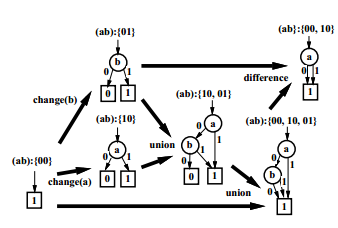
\includegraphics[scale=.90]{construction}
\caption{Construction of ZBDDs for sets of combination \cite{minato2001zero}}.
\label{fig:construction}
\end{figure}

ZBDDs support many operations for sets of combinations. Some of the basic operations that can be performed are shown here. In the following, \textbf{P} and \textbf{Q} indicate the instances of sets of combinations represented by ZBDDs and \textbf{v} means an input variable. The flowchart shown in Figure \ref{fig:construction} is the method in which the polynomials can be built. Here the polynomials are treated as sets. Any set of combinations can be generated by a sequence of these basic operations. In ZBDDs there is no support for the unary complement operation but it is essential in OBDDs. In case there is a need to compute the complement we first define a universal set \textbf{U} to compute complement set $\bar{P}$ and then use the difference operation $(\textbf{U} - \bar{P})$ to compute it \cite{minato2001zero}.

\begin{align*}
&``{\O}``           &\text{the empty set. (0-terminal node.) } \ \ \ \ \ \\
&``\textbf{1}``     &\text{the set of only the null combination	} \ \\
&                   &\{ 0 0 \ldots 0 \}.\ \text{(1-terminal node.)} \ \ \ \ \ \ \ \ \ \ \ \\
%&P\text{.top}       &\text{the variable at the root of the ZBDD.} \\
%&P\text{.offset}(v) &\text{selects the subset of the combinations} \\
%&                   &\text{each of which does not include }v \ \ \ \ \ \\
%&P\text{.onset}(v)  &\text{selects the subset of the combinations} \\
%&					&\text{including } v,\text{ and then delete } v \text{ from} \ \ \ \\
%&					&\text{each combination.} \ \ \ \ \ \ \ \ \ \ \ \ \ \ \ \ \ \ \ \ \ \ \ \\
&P\text{.change}(v) &\text{inverts } v \text{ on each combination.(swaps} \ \\
&					&\text{onset and offset of } P.) \ \ \ \ \ \ \ \ \ \ \ \ \ \ \ \ \ \ \\
&P \cup Q			&\text{the union set of } P \text{ and } Q. \ \ \ \ \ \ \ \ \ \ \ \ \ \ \\
&P \cap Q			&\text{the intersection set of } P \text{ and } Q. \ \ \ \ \ \ \ \\
&P - Q				&\text{the difference set.(combinations in } P \ \\
&					&\text{but not in } Q.) \ \ \ \ \ \ \ \ \ \ \ \ \ \ \ \ \ \ \ \ \ \ \ \ \ \ \ \ 
\end{align*}
\section{Algorithms}
\label{sec:algorithms}
In order to run Buchberger's algorithm, we need to formulate helper functions.  These functions have to be able to process ZBDDs and return the correct object.  The first algorithm is to find leading terms in a ZBDD.  The algorithm loops through the ZBDD object by traversing the ``then`` child (also known as the 1  path).  The function returns a pointer to a DdNode that represents the leading terms of the ZBDD function.
{\small
\begin{align*}
&\textbf{Inputs:}\ \ DdManager,\ ZBDD,\ Variable List[\ ],\ 1 \\
&\textbf{Outputs:}\ Leading\ Terms \\
&\ \ \text{1: }\ temp\leftarrow 1; \\
&\ \ \text{2: }\ \textbf{int } i = index of ZBDD; \\
&\ \ \text{2: }\ \textbf{while }(ZBDD\neq \textbf{Const. Node})\ \textbf{do} \\
&\ \ \text{3: }\ \ \ temp\ =\ VariableList[i]*temp \\
&\ \ \text{4: }\ \ \ ZBDD\ =\ then\ child\ of\ ZBDD \\
&\ \ \text{5: }\ \ \ i\ =\ i + 1 \\
&\ \ \text{6: }\ \textbf{end while} \\
&\ \ \text{7: }\ \text{return } temp;
\end{align*}
\par}

The next algorithm is multivariate division.  Again, this function had to be adapted to return a pointer to a DdNode that represents the remainder of the division as a ZBDD.  The ZBDD input is the dividend and the ZBDDlist is the divisor.  The ZBDDlist is a struct that includes a DdNode pointer and a pointer to the next DdNode in the list.  The algorithm loops through each DdNode in the list, finds the leading term and then attempts to divide the ZBDD.
{\small
\begin{align*}
&\textbf{Inputs:}\ \ DdManager,\ ZBDD,\ ZBDDlist[\ ],\ Variable List[\ ],\ 1 \\
&\textbf{Outputs:}\ Remainder \\ 
&\ \ \text{1: }\ zero\leftarrow 0;\ quot\leftarrow 0;\ rem\leftarrow 0; \\
&\ \ \text{2: }\ \textbf{int } i = 1; \\
&\ \ \text{3: }\ \textbf{while } (ZBDD \neq zero)\ \textbf{do} \\
&\ \ \text{4: }\ \ \ \textbf{if } \exists i\ \text{s.t.} \frac{LT(ZBDD)}{LT(ZBDDlist[i])} \textbf{then} \\
&\ \ \text{5: }\ \ \ \ \ quot =\lbrace\left (quot \cup \frac{LT(ZBDD)}{LT(ZBDDlist[i])} \right)\\
&\ \ \ \ \ \ \ \ \ \ \ \ \ \ \ \ \ -\ \left( quot \cap \frac{LT(ZBDD)}{LT(ZBDDlist[i])} \right)\rbrace \\
&\ \ \text{6: }\ \ \ \ \ ZBDD = \{ZBDD\} - \left\lbrace\frac{LT(ZBDD)}{LT(ZBDDlist[i])}\right\rbrace*ZBDDList[i] \\
&\ \ \text{7: }\ \ \ \textbf{else } \\
&\ \ \text{8: }\ \ \ \ \ rem = \left(rem \cup LT(ZBDD)\right) - \left(rem\cap LT(ZBDD)\right) \\
&\ \ \text{9: }\ \ \ \ \ ZBDD = \{ZBDD\} - \{LT(ZBDD)\} \\
&\ \text{10: }\ \ \ \textbf{end if } \\
&\ \text{11: }\ i = i+1; \\
&\ \text{12: }\ \textbf{end  while} \\
&\ \text{13: }\ \text{return } rem; \\
\end{align*}
\par}

One of the key steps in Buchberger's algorithm is finding the s-polynomials of the functions.  S-polynomials are formed to cancel the leading terms of two polynomials.  The Gr{\H o}bner basis can be directly defined by these s-polynomials. 
{\small
\begin{align*}
&\textbf{Theorem } Let\ I \subset K\left[ x_{1},x_{2},\ldots ,x_{n}\right] \ be\ a\ polynomial\ ideal \\ &with\ basis\ G = \{ g_{1},g_{2},\ldots ,g_{n} \} \ then\ G\ is\ a\ Gr\text{{\H o}}bner\ basis \\ 
&for\ I\ if\ and\ only\ if\ the\ remainder\ on\ dividing\ every\ S- \\
&polynomial\ S\left(g_{i},g_{j}\right)\left(i \not= j \right)\ by\ G\ ( in\ any\ order\ of\ the \\ 
&basis\ elements ) \ is\ zero. \cite{seligspoly} 
\end{align*}
\par} 

Here is the algorithm for computing s-polynomials on ZBDDs.

{\small
\begin{align*}
&\textbf{Inputs:}\ \ DdManager,\ ZBDD1,\ ZBDD2,\ VariableList[\ ],\ 1 \\
&\textbf{Outputs:}\ S-polynomial \\
&\ \ \text{1: }\ LCM = LT(ZBDD1)*LT(ZBBD2) \\
&\ \ \text{2: }\ prod1 = \frac{LCM}{LT(ZBDD1)}ZBBD1 \\
&\ \ \text{3: }\ prod2 = \frac{LCM}{LT(ZBDD2)}ZBBD2 \\
&\ \ \text{4: }\ prod3 = prod1 \cap prod2 \\
&\ \ \text{5: }\ \textbf{if } prod1 \ge prod2\ \textbf{then} \\
&\ \ \text{6: }\ \ \ diff = \{prod2\} - \{prod3\} \\
&\ \ \text{7: }\ \ \ sply = \{prod1\} - \{prod2\} \\
&\ \ \text{8: }\ \ \ sply = \left(sply \cup diff\right) - \left(sply \cap diff\right) \\
&\ \ \text{9: }\ \textbf{else } \\
&\ \text{10: }\ \ \ diff = \{prod1\} - \{prod3\} \\
&\ \text{11: }\ \ \ sply = \{prod2\} - \{prod1\} \\
&\ \text{12: }\ \ \ sply = \left(sply \cup diff\right) - \left(sply \cap diff\right) \\
&\ \text{13: }\ \textbf{end if } \\
&\ \text{14: }\ \text{return } sply; \\
\end{align*}
\par}

With the help of the above mentioned functions, Buchberger's algorithm can be run on ZBDDs.  The function below repeatedly computes the s-polynomials of pairs of ZBDDs and then divides by the list of ZBDDs.  If the remainder is non-zero then the remainder is added to the list of ZBDDs.  The algorithm is shown below. 
{\small
\begin{align*}
&\textbf{Inputs:}\ \ F = List\ of\ ZBDDs \\
&\ \ \ \ \ \ \ \ \ \ \left[ f_{1},f_{2},\ldots ,f_s \right] \\
&\textbf{Outputs:}\ G = List\ of\ ZBDDs\ representing\ the\ Gr\text{{\H o}}bner\ basis \\
&\ \ \ \ \ \ \ \ \ \ \ \left[ g_{1},g_{2},\ldots ,g_t \right]\\
&\ \ \text{1: }\ \text{Initialize: } G:=F;\ \mathcal{G}:=\{\{f_i , f_j\} \mid f_i \not= f_j \in G\} \\  
&\ \ \text{2: }\ \textbf{while } \mathcal{G} \not= {\O}\ \textbf{do} \\
&\ \ \text{3: }\ \ \ \text{Pick a pair } \{ f, g\} \in \mathcal{G} \\
&\ \ \text{4: }\ \ \ \mathcal{G} := \{ \mathcal{G} \} - \{\{f,g\}\} \\
&\ \ \text{5: }\ \ \ Spoly(f,g)\overset{G}{\to} +\ h \\
&\ \ \text{6: }\ \ \ \textbf{if } h \not= 0\ \textbf{then} \\
&\ \ \text{7: }\ \ \ \ \ \ \mathcal{G} := \mathcal{G} \cup \{\{u,h\} \mid \forall u \in G\} \\ 
&\ \ \text{8: }\ \ \ \ \ \ G := \left( G \cup h \right) - \left( G \cap h \right) \\
&\ \ \text{9: }\ \ \ \textbf{end if} \\
&\ \text{10: }\ \textbf{end while} \\
\end{align*}
\par}

Once the Gr{\H o}bner basis has been computed, further simplification and elimination of terms can be performed.  The minimal form of a Gr{\H o}bner basis has a leading coefficient of 1 in each of the functions representing the basis.  Since we are only working with variables and no coefficients this step is not necessary in our computations.  The second step in finding the minimal form is to remove sets from the basis that contain the same leading terms.  This can be performed by looping through all pairs of leading terms and deleting if they are equal.

The final step in computing the Gr{\H o}bner basis is to reduce the set of functions.  The basis can be further reduced by performing multivariate division on each function in the basis.  The algorithm is described below.
{\small
\begin{align*}
&\textbf{Inputs:}\ \ G = List\ of\ ZBDDs\ representing\ the\ minimal\ Gr\text{{\H o}}bner\ basis \\
&\ \ \ \ \ \ \ \ \ \ \left[ g_{1},g_{2},\ldots ,g_s \right] \\
&\textbf{Outputs:}\ R = List\ of\ ZBDDs\ representing\ the\ reduced\ Gr\text{{\H o}}bner\ basis \\
&\ \ \ \ \ \ \ \ \ \ \ \left[ r_{1},r_{2},\ldots ,r_t \right]\\
&\ \ \text{1: }\ R \leftarrow 0 \\
&\ \ \text{2: }\ \forall g_{i},g_{j} \in G \textbf{ where } i \not= j \\
&\ \ \text{3: }\ remainder = \frac{g_{i}}{g_{j}} \\
&\ \ \text{4: }\ \textbf{if } \{ remainder \not= 0 \} \textbf{ then} \\
&\ \ \text{5: }\ \ \ R = R \cup remainder \\
&\ \ \text{6: }\ \textbf{end if} \\
&\ \ \text{7: }\ \text{return } R
\end{align*}
\par}
\section{The Experiment}
\label{sec:experiment}
We set out to perform Buchberger's algorithm to ZBDDs.  The purpose was to test if we could properly find the Gr{\H o}bner basis of a polynomial that was represented by a ZBDD.  Three experiment sets were performed to test the functionality of our code.

\subsection{Case 1}
\label{sec:case1}
\begin{align*}
\textbf{Cyclic Polynomials: } \\
f_{1} &= x_{1}+x_{2}+x_{3}+x_{4} \\
f_{2} &= x_{1}x_{2}+x_{2}x_{3}+x_{3}x_{4}+x_{4}x_{1} \\
f_{3} &= x_{1}x_{2}x_{3}+x_{2}x_{3}x_{4}+x_{3}x_{4}x_{1}++x_{4}x_{1}x_{2}\\
f_{4} &= x_{1}x_{2}x_{3}x_{4}-1
\end{align*}
Cyclic polynomials were used to test the code. Here the order maintained is the lexicographic order with (x1,x2,x3,x4). The reduced Gr{\H o}bner basis generated from the output of our code are in the form of minterms \{ X000 1 , 0X00 1, 00X0 1, 000X 1 \} which are $x_{1} + 1, x_{2} + 1, x_{3} + 1, x_{4} + 1$ when compared to the input polynomials. Figure \ref{fig:case1} shows the ZBDD representation of the reduced Gr{\H o}bner basis obtained using the GraphViz tool.

\begin{figure}[b]\centering
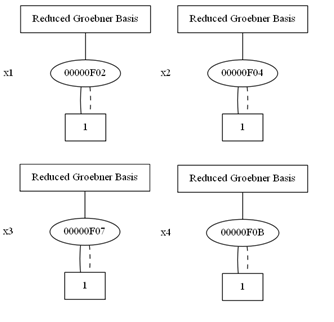
\includegraphics[scale=.90]{case1}
\caption{ZBDD representation of reduced Gr{\H o}bner Basis for cyclic polynomials.}
\label{fig:case1}
\end{figure}

\subsection{Case 2}
\label{sec:case2}
\begin{align*}
\textbf{More Polynomials: } \\
f_{1} &= ab+1 \\
f_{2} &= ab+a+1 \\
f_{3} &= ab+b+1 \\
f_{4} &= ab+a+b \\
f_{5} &= xy+x+y \\
f_{6} &= yz+y+z
\end{align*}
We also tested the code with the use of another set of polynomials with the lexicographic order (x,y,z,a,b). The reduced Gr{\H o}bner basis generated from the code are in the form of minterms 00000 1. Figure \ref{fig:case2} shows the ZBDD representation of reduced Gr{\H o}bner basis obtained using the GraphViz tool.

\begin{figure}[t]\centering
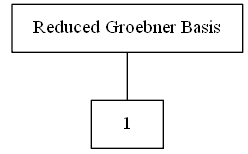
\includegraphics[scale=.75]{case2}
\caption{ZBDD representation of reduced Gr{\H o}bner Basis for more polynomials.}
\label{fig:case2}
\end{figure}

\subsection{Case 3}
\label{sec:case3}
\begin{align*}
\textbf{Chain of OR Gates: } \\
f_{1} &= z+he+h+e \\
f_{2} &= h+gd+g+d \\
f_{3} &= g+f+c+cf \\
f_{4} &= f+a+b+ab \\
\end{align*}

In arithmetic circuits with a chain of OR gates (Figure \ref{fig:case3}), the reduction process is a big problem.  Reduction leads to the generation of a huge number of new monomials and the process takes a long time to complete.  We tried reduction (our multivariate division in Singular) of z with the set of equations $f_{1},f_{2},f_{3},f_{4}$. It took 10ms in Singular and it took 1ms with our c code.

\begin{figure}[b]\centering
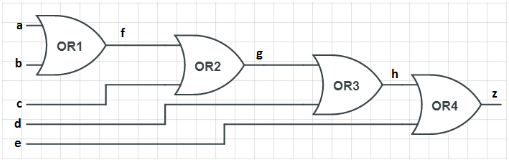
\includegraphics[scale=.6]{case3}
\caption{Top level model of chain of OR gates.}
\label{fig:case3}
\end{figure}

\section{Problems Faced and its Potential Solutions}
\label{sec:problems}
A few problems were encountered while writing and testing the ZBDD code.  Initially we declared the ZBDD variables by using the function cudd\_ZddIthvar, but we were not able to perform basic operations such as union and intersection properly. We also had the problem of getting extra nodes while generating ZBDDs.  Later, after discussing with the professor about the problem, we understood that we needed to look at ZBDDs as sets. This eliminated all the problems and all the operations such as difference, intersection were working fine.  After running several sets of polynomials everything was found to be working fine. When we tried using the cyclic polynomials we found that we had a bug in the code relating to the union operation. We wanted to use the union operation as an addition operation and therefore expected the result of 001 $\cup$ 001 to be zero, instead the result was 001. Since we are operating in the Boolean domain we had to modify the union operation to get zero. We had to replace the union operation in terms of the intersection i.e., $$ A + B = (A \cup B)-(A \cap B)$$ and also we were using the inbuilt cudd\_ZddunateProduct which internally uses the union operation so we modified it accordingly. With the help of these two steps bug was successfully removed.

\section{Conclusion}
\label{sec:conc}
ZBDDs are an efficient method to solve formal verification.  In terms of size in memory, ZBDDs are a  simplified version of BDDs therefore taking less system space.  \ref{sec:case3} shows that we were also able to generate reduction in a more timely fashion.  As demonstrated, the buchberger's algorithm can be modified to work on ZBDDs to find the Gr{\H o}bner basis on the sets of combinations.  With a little more time and a program that can generate ZBDDs from functions, we believe that our code generates the correct Gr{\H o}bner basis for sets of ZBDDs.    

\section{Contributions}
\label{sec:cont}
Harsha Gadiraju was involved in the writing of the major part of the code such as the successful creation of lists using the linked lists, figuring the leading term, S-polynomial and Buchberger’s algorithm. Revanth Rajalbandi was involved in the writing of the reduced and minimal Gr{\H o}bner Basis, helped Harsha while writing the code, researching the information out of the Journal papers and debugging the code by solving the Gr{\H o}bner basis manually on the paper. Ian Noy was involved in figuring out the problems in the multivariate division, conversion of leading terms and multivariate division into functions and he spent a lot time in our initial attempts to create ZBDDs.

Other contributions come from the information gathered from scholarly resources. Shin-ichi Minato wrote three very good papers on BDDs and ZBDDs \cite{minato2001zero,minato1993zero,minato1996binary}.  He is regarded as one of the key researchers in ZBDDs. 

%%%%%%%%%%%%%%%%%%%%%%%%%%%%%%%%%%%%%%%%%%%%%%%%%%%%%%%%%%%%%%%%%%%%%%%%%%%%%%%%
%\begin{multicols}{2}
\bibliographystyle{IEEEtran}
\bibliography{ece5745bib}
%\end{multicols}


\end{document}


% LocalWords:  tikz pt greenbox darkgreen lightgreen ra lightblue tikzpicture
